\chapter{Diagramme SQL}

La page suivante contient le diagramme SQL de notre base de données. Ce dernier
a été crée avec le logiciel DBSchema \cite{dbschema}.

On voit bien la distinction entre notre base de données, vbMifare, et celle de
Polytech. Nous interagissons avec la table Users de cette dernière.

    \begin{figure}[h]
        \begin{center}
            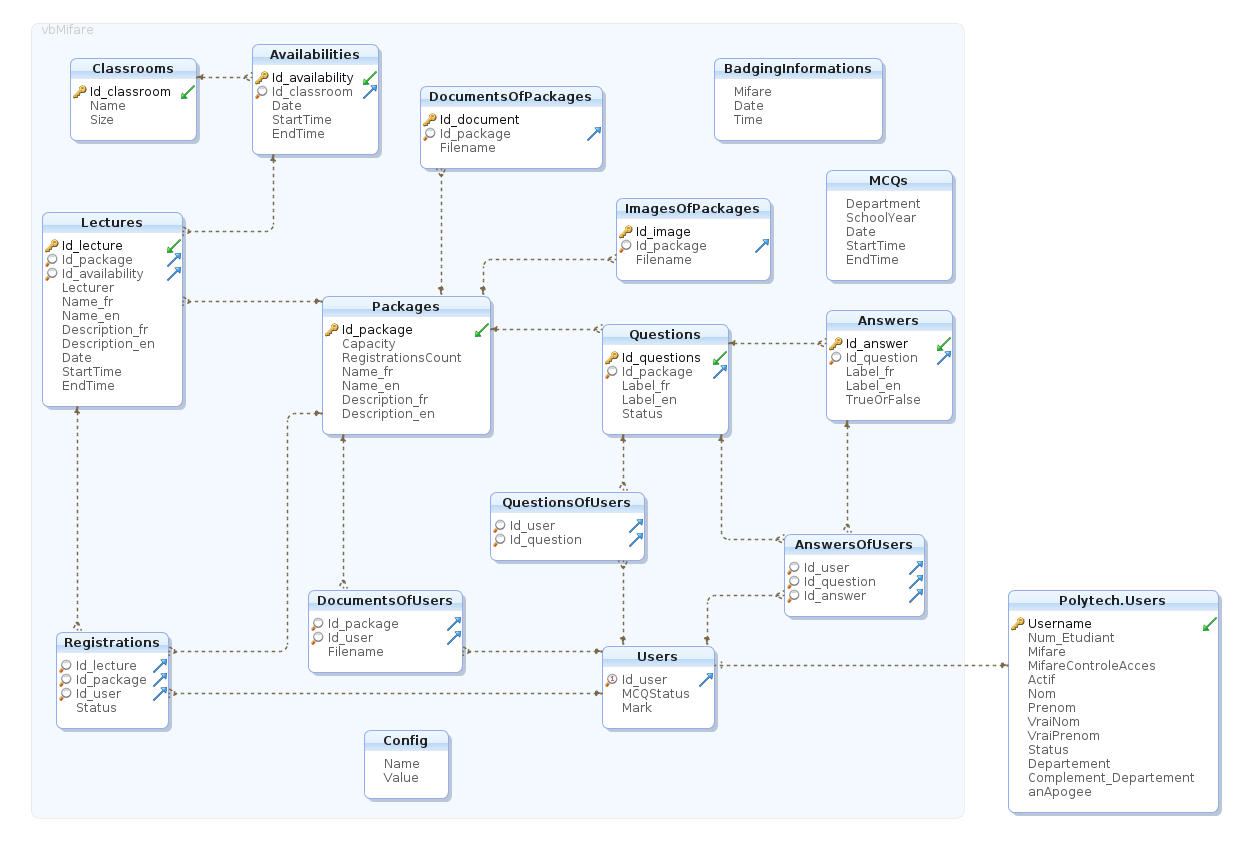
\includegraphics[angle=90, scale=0.54]{images/sql.png} 
        \end{center}

        \caption{Diagramme SQL}
        \label{Diagramme SQL}
    \end{figure}
